\chapter{Rasteryzacja sceny}
\thispagestyle{chapterBeginStyle}
\section{Opis procesu}

Wszystkie dane, które są dostępne do wnioskowania na temat sceny znajdują się we wcześniej omawianych czterech tablicach \texttt{zarr}. Krokiem, który jest niezbędny, aby algorytm działał z wysoką skutecznością jest odpowiednie przygotowanie danych. Każda scena zawiera obiekty. Liczba tych obiektów może się zmieniać, tak samo jak struktura tych obiektów, gdyż nie są to obiekty tej samej klasy. Aby móc zastosować te informacje do wnioskowania za pomocą sieci neuronowych, trzeba te dane przetworzyć w sposób taki, który umożliwia przeprowadzenie procesu uczenia w sposób ustandaryzowany (z założeniami na temat tego jak dane wejściowe wpływają na dane wyjściowe funkcji przetwarzającej je). W tym rozdziale omówiony jest jeden ze sposobów przetwarzania danych, czyli rasteryzacja. Rasteryzacja polega na przetworzeniu sceny (wszystkich informacji na jej temat dostępnych) do formy obrazu. W tej pracy obrazy przedstawiające scenę ukazane są w widoku \texttt{BEV} (widok z lotu ptaka).

\section{Rasteryzator \texttt{SemBoxRasterizer}}

\begin{figure}[htbp]
    \centering
    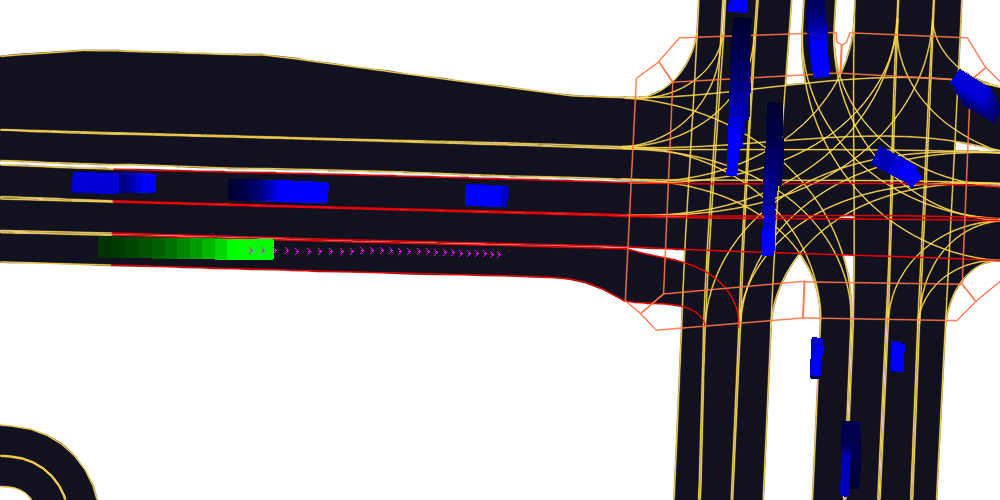
\includegraphics[width=\linewidth]{raster_l5kit.png}
    \caption{Wizualizacja rasteryzatora \texttt{SemBoxRasterizer}}
\end{figure}

\newpage

Biblioteka \texttt{l5kit} posiada klasę \texttt{SemBoxRasterizer}, która pozwala rasteryzować dane bez konieczności własnej implementacji rasteryzatora. Klasa \texttt{SemBoxRasterizer} posiada rozwiązania, które mogą znacząco wpływać na skuteczność predykcji np. kolorowanie historycznych pozycji ciemniejszymi kolorami (im wcześniejsza tym ciemniejsza), zaznaczanie pozycji przejść dla pieszych, zaznaczanie krawędzi prawej oraz lewej pasa w każdym miejscu (nawet na skrzyżowaniach, co jest czasem trudne w interpretacji). Następny rasteryzator posiada rozwiązania, które mają za zadanie uprościć rasteryzowany obraz w nadzieji na to, że modele uczące się na tych obrazach będą uczyć się szybciej i dokładniej.

\section{Rasteryzator \texttt{CenterLines}}

\begin{figure}[htbp]
    \centering
    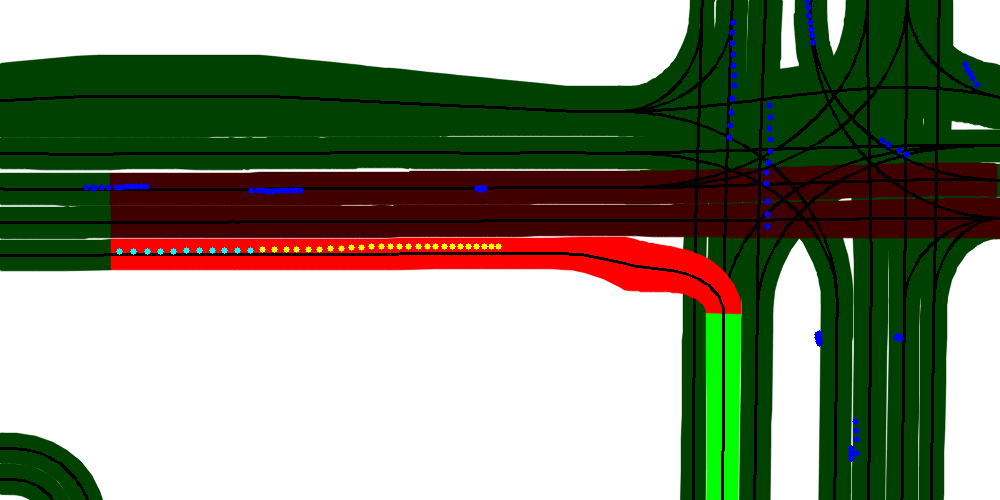
\includegraphics[width=\linewidth]{raster_custom.png}
    \caption{Wizualizacja rasteryzatora \texttt{CenterLines}}
\end{figure}

Rasteryzator CenterLines został zaprojektowany mając na uwadze maksymalne uproszczenie rasteryzowanej sceny, co potencjalnie mogłoby wpłynąć pozytywnie na skuteczność predykcji. Rzeczy które zostały zrobione inaczej w tym rasteryzatorze:

\begin{itemize}
    \item Agenci zaznaczeni są jako kropki o stałym rozmiarze, bez zaznaczania wcześniejszych pozycji ciemniejszym kolorem (uproszczenie, które miało na celu ułatwienie procesu trenowania)
    \item Wejściowe pozycje agenta \texttt{EGO} są zaznaczone kolorem seledynowym, pozycje wyjściowe są zaznaczone na żółto. Ważne jest, że pozycje wyjściowe są tylko poglądowe (nie występują ani w zbiorze treningowym, ani w zbiorze testowym). Tak więc nie mają w żadnym stopniu wpływu na proces trenowania i przewidywania.
    \item Nie występują krawędzie prawa i lewa zaznaczone odpowiednimi kolorami, te krawędzie zostały zastąpione pasem pokolorowanym na zielono, jeśli światła wskazują, że można nim jechać, lub czerwonym w przeciwnym wypadku. Krawędzie prawa i lewa zostały połączone w krawędź środkową pasa. Krawędź ta wyznacza możliwe kierunki w jakich może się poruszać agent.
    \item Pasy, które są osiągalne dla agenta \texttt{EGO} bez zmiany pasa z aktualnej pozycji, zostały wyróżnione jaśniejszymi kolorami, te do których agent \texttt{EGO} nie może dotrzeć bez zmiany pasa zostały zaciemnione.
\end{itemize}

\newpage

\section{Algorytm wyznaczania środka pasa \texttt{AWSP}}

Do wyznaczenia środka pasa na podstawie prawej i lewej krawędzi został zaimplementowany algorytm interpolujący \texttt{AWSP}. Algorytm został opisany w pseudokodzie, a samo działanie algorytmu zostało przedstawione na wykresach dotyczących przykładowego kawałka pasa ruchu.

\subsection{Opis danych wejściowych i wynikowych}

\vspace{0em}
\begin{minted}{python}
lane_in = {
    'xyz_left': np.array([[x_0, y_0, z_0], ... [x_n, y_n, z_n]]),   # lewa krawędź
    'xyz_right': np.array([[x_0, y_0, z_0], ... [x_m, y_m, z_m]]),  # prawa krawędź
    'lights': lights_color                                          # sygnalizacja pasa
}

lane_out = {
    'xy_left': np.array([[x_0, y_0], ... [x_n, y_n]]),              # lewa krawędź
    'xy_right': np.array([[x_0, y_0], ... [x_m, y_m]]),             # prawa krawędź
    'xy_center': np.array([[x_0, y_0], ... [x_k, y_k]]),            # środkowa krawędź
    'lights': lights_color                                          # sygnalizacja pasa
}
\end{minted}

\subsection{Pseudokod algorytmu \texttt{AWSP}}

\begin{pseudokod}[H]
    \SetAlgoLined
    \DontPrintSemicolon
    \textbf{Dane wejściowe:} $lane\_in$\;
    \textbf{Dane wynikowe:} $lane\_out \leftarrow \{\;\}$\;
    
    \BlankLine
    \For{$side$ $\in$ \text{\upshape \lbrack}$left$, $right$\text{\upshape \rbrack}}{
        $d \leftarrow pairwise\_L2\_norm(lane\_in['xyz\_side'])$\Comment*[r]{Odległości sąsiednich węzłów interpolacji krawędzi}
        $d \leftarrow cumulative\_sum(d)$\Comment*[r]{Odległości od pierwszego węzła interpolacji}
        $side\_l \leftarrow d[-1]$\Comment*[r]{Długość krawędzi (odległość od pierwszego węzła do ostatniego)}
        $t \leftarrow d / max(d)$\Comment*[r]{Wektor rosnących wartości parametru $t \in [0, 1]$}
        $side\_fx \leftarrow interpolating\_f(t,lane\_in['xyz\_side']['x'])$\Comment*[r]{Funkcja $x(t)$ danej krawędzi}
        $side\_fy \leftarrow interpolating\_f(t,lane\_in['xyz\_side']['y'])$\Comment*[r]{Funkcja $y(t)$ danej krawędzi}
    }
    
    \BlankLine
    $n \leftarrow \lceil max(left\_l, right\_l) / 0.5 \rceil$\Comment*[r]{Optymalna ilość węzłów interpolacji}
    $t \leftarrow \lbrack 0, 1, ... , n-1, n \rbrack/n$\Comment*[r]{Wartości węzłów interpolacji}
    
    \BlankLine
    \For{$side$ $\in$ \text{\upshape \lbrack}$left$, $right$\text{\upshape \rbrack}}{
        $side\_xy \leftarrow [side\_fx(t), side\_fy(t)]$\Comment*[r]{Interpolowane wartości współrzędnych xy danej krawędzi}
    }
    
    \BlankLine
    $lane\_out['xy\_center'] \leftarrow (left\_xy + right\_xy)/2$\Comment*[r]{Środek pasa to ciąg punktów środkowych}
    $lane\_out['xy\_right'] \leftarrow lane\_in['xyz\_right']['xy']$\;
    $lane\_out['xy\_left'] \leftarrow lane\_in['xyz\_left']['xy']$\;
    $lane\_out['lights'] \leftarrow lane\_in['lights']$\;
    
    \BlankLine
    \textbf{return} $lane\_out$

    \caption{Algorytm AWSP}
\end{pseudokod}

\newpage

\subsection{Wizualizacja algorytmu \texttt{AWSP}}

\begin{figure}[H]
    \centering
    \subfloat[Współrzędna x środka pasa w zależności od parametru t]{\includesvg[width=0.5\textwidth]{center_lane_vis_1.svg}}
    \subfloat[Współrzędna y środka pasa w zależności od parametru t]{\includesvg[width=0.5\textwidth]{center_lane_vis_2.svg}}
\end{figure}

\begin{figure}[H]
    \centering
    \subfloat[Węzły interpolacji rozważanego kawałka pasa jezdni]{\includesvg[width=0.5\textwidth]{center_lane_vis_0.svg}}
    \subfloat[Uzyskany środek pasa ruchu]{\includesvg[width=0.5\textwidth]{center_lane_vis_3.svg}}
\end{figure}

\newpage

\subsection{Implementacja algorytmu \texttt{AWSP}}

\vspace*{0.5cm}

\begin{minted}{python}
import numpy as np
from scipy.interpolate import interp1d

def algorithm_awsp(lane_in):
    lights = lane_in['lights'] # kolor świateł
    lane_l = lane_in['xyz_left'][:, :2] # współrzędne xyz węzłów lewej krawędzi pasa
    lane_r = lane_in['xyz_right'][:, :2] # współrzędne xyz węzłów prawej krawędzi pasa
    # współrzędne węzłów lane_l oraz lane_r są przedstawione na rysunku (c)
    
    # odległości pomiędzy kolejnymi węzłami
    lane_l_dist = np.linalg.norm(lane_l[1:] - lane_l[:-1], axis=1)
    lane_l_dist = np.cumsum(lane_l_dist) # odległości po krawędzi do pierwszego węzła
    l_total_dist = lane_l_dist[-1] # długość krawędzi
    lane_l_dist = np.concatenate([[0], lane_l_dist]) # uwzględnienie pierwszego węzła
    lane_l_t = lane_l_dist / lane_l_dist[-1] # wyznaczenie parametru t dla każdego węzła

    lane_r_dist = np.linalg.norm(lane_r[1:] - lane_r[:-1], axis=1)
    lane_r_dist = np.cumsum(lane_r_dist)
    r_total_dist = lane_r_dist[-1]
    lane_r_dist = np.concatenate([[0], lane_r_dist])
    lane_r_t = lane_r_dist / lane_r_dist[-1]

    # inicjalizacja funkcji interpolujących liniowo współrzędne węzłów w zależności od t
    l_x_interp = interp1d(lane_l_t, lane_l[:, 0]) 
    l_y_interp = interp1d(lane_l_t, lane_l[:, 1])
    r_x_interp = interp1d(lane_r_t, lane_r[:, 0])
    r_y_interp = interp1d(lane_r_t, lane_r[:, 1])

    # liczba węzłów krawędzi środkowej (minimum 1 węzeł na 0.5m, w sumie minimum 3 węzły)
    steps = max(int(np.ceil(max(l_total_dist, r_total_dist) / 0.5)), 3)
    # wektor wartości parametru t, używany do wyliczenia węzłów krawędzi środkowej
    steps_vec = np.arange(steps)/(steps - 1)

    # obliczanie współrzędnych x krawędzi środkowej, przedstawione na rysunku (a)
    mid_points_x = (l_x_interp(steps_vec) + r_x_interp(steps_vec)) / 2.0
    
    # obliczanie współrzędnych y krawędzi środkowej, przedstawione na rysunku (b)
    mid_points_y = (l_y_interp(steps_vec) + r_y_interp(steps_vec)) / 2.0
    
    # współrzędne xy krawędzi środkowej, przedstawione na rysunku (d)
    mid_points = np.stack([mid_points_x, mid_points_y], axis=0).T

    lane_out = {
        'xy_left': lane_l,
        'xy_right': lane_r,
        'xy_center': mid_points,
        'lights': lights
    }

    return lane_out
\end{minted}


\newpage

\section{Algorytm wyznaczania osiągalnych pasów \texttt{AWOP}}

W rasteryzatorze \texttt{CenterLines} pasy, które są osiągalne przez agenta \texttt{EGO} bez zmiany pasa są zaznaczone jaśniejszym kolorem. Aby takie kolorowanie było możliwe trzeba najpierw wyznaczyć te pasy. Dla każdej sceny możliwe jest uzyskanie listy wszystkich pasów zawartych przynajmniej częściowo na tej scenie. Dla każdego elementu z tej listy (pas drogowy), wyznaczany jest następnie środek pasa za pomocą algorytmu \texttt{AWSP}. Elementy te można następnie wykorzystać do zbudowania reprezentacji grafowej mapy za pomocą algorytmu \texttt{AWOP}. Kąt odchylenia najbliższego pasa będzie przydatny w dalszych etapach podczas normalizacji sceny.

\subsection{Opis danych wejściowych i wynikowych}

\vspace{0em}
\begin{minted}{python}
lanes_in = [                                                  # lista pasów ruchu
    {
        'xy_left': np.array([[x_0, y_0], ... [x_n, y_n]]),    # lewa krawędź
        'xy_right': np.array([[x_0, y_0], ... [x_m, y_m]]),   # prawa krawędź
        'xy_center': np.array([[x_0, y_0], ... [x_k, y_k]]),  # środkowa krawędź
        'lights': lights_color                                # sygnalizacja na pasie
    },
    ...
]

agent_ego_in = np.array([                                     # wejściowe współrzędne
    [x_0, y_0],                                               # agenta EGO
    ...                                                       # lista 11 punktów xy
    [x_10, y_10]
])

lanes_out = [                                                 # lista pasów ruchu
    {
        'xy_left': np.array([[x_0, y_0], ... [x_n, y_n]]),    # lewa krawędź
        'xy_right': np.array([[x_0, y_0], ... [x_m, y_m]]),   # prawa krawędź
        'xy_center': np.array([[x_0, y_0], ... [x_k, y_k]]),  # środkowa krawędź
        'lights': lights_color,                               # sygnalizacja na pasie
        'reachable': lane_reachability_status                 # True/False status
    },                                                        # osiągalności pasa
    ...
]

yaw_out = agent_ego_closest_lane_yaw                          # kąt odchylenia pasa
                                                              # najbliższego agentowi EGO
\end{minted}

\subsection{Pseudokod algorytmu \texttt{AWOP}}

\begin{pseudokod}[H]
    \SetAlgoLined
    \DontPrintSemicolon
    \textbf{Dane wejściowe:} $lanes\_in, agent\_ego\_in$\;
    \textbf{Dane wynikowe:} $lanes\_out, yaw\_out$\;
    
    \BlankLine
    $lanes\_out \leftarrow get\_graph\_representation(lanes\_in)$\Comment*[r]{Przypisanie każdemu pasowi 2 wierzchołków grafu}
    $idx \leftarrow get\_ego\_closest\_lane(lanes\_out, agent\_ego\_in)$\Comment*[r]{Pas najbliższy pozycjom wejściowym agenta EGO}
    $lanes\_out \leftarrow get\_reachability(lanes\_out, idx)$\Comment*[r]{Dodanie do pasów informacji o osiągalności}
    $yaw\_out \leftarrow get\_closest\_lane\_yaw(lanes\_out, agent\_ego\_in, idx)$\Comment*[r]{Kąt odchylenia najbliższego pasa}
    
    \BlankLine
    \textbf{return} $lanes\_out, yaw\_out$

    \caption{Algorytm AWOP}
\end{pseudokod}

\newpage

\subsection{Funkcje pomocnicze algorytmu \texttt{AWOP}}

\subsubsection{Pseudokod funkcji \texttt{get\_graph\_representation}}

\begin{pseudokod}[H]
    \SetAlgoLined
    \DontPrintSemicolon
    \textbf{Dane wejściowe:} $lanes\_list$\;
    \textbf{Dane wynikowe:} $lanes\_list$\;
    
    \BlankLine
    $nodes \leftarrow \lbrack\;\rbrack$\;
    $unique\_nodes \leftarrow \lbrack\;\rbrack$\;
    
    \BlankLine
    \For{$lane$ $\in$ $lanes\_list$}{
        $nodes.append(lane['xy\_center'].first)$\Comment*[r]{Pierwszy węzeł interpolacji jako wierzchołek grafu}
        $nodes.append(lane['xy\_center'].last)$\Comment*[r]{Ostatni węzeł interpolacji jako wierzchołek grafu}
    }
    
    \BlankLine
    \For{$node$ $\in$ $nodes$}{
        \uIf{$len(nodes) == 0\:\textbf{\upshape or}\:min\_distance(unique\_nodes, node) < \epsilon$}{
            $unique\_nodes.append(node)$\Comment*[r]{Jest dodany jeśli nie ma podobnego wierzchołka w liście}
        }
    }
    
    \BlankLine
    \For{$lane$ $\in$ $lanes\_list$}{
        $lane['node\_0'] \leftarrow closest\_idx(unique\_nodes, lane['xy\_center'].first)$\Comment*[r]{Indeks najbliższego wierzchołka}
        $lane['node\_1'] \leftarrow closest\_idx(unique\_nodes, lane['xy\_center'].last)$\Comment*[r]{Indeks najbliższego wierzchołka}
    }
    
    \BlankLine
    \textbf{return} $lanes\_list$

    \caption{Funkcja get\_graph\_representation}
\end{pseudokod}

\subsubsection{Implementacja funkcji \texttt{get\_graph\_representation}}

\begin{minted}{python}
def graph_representation(lanes_list):
    nodes = []
    unique_nodes = []

    for lane in lanes_list:
        nodes.append(lane['xy_center'][0])
        nodes.append(lane['xy_center'][-1])

    for node in nodes:
        if len(unique_nodes) == 0:
            unique_nodes.append(node)
        elif np.min(np.linalg.norm(np.array(unique_nodes) - node, axis=1)) > 0.1:
            unique_nodes.append(node)

    for lane in lanes_list:
        lane['node_0'] = np.argmin(np.linalg.norm(
            np.array(unique_nodes) - lane['xy_center'][0], axis=1
        ))
        lane['node_1'] = np.argmin(np.linalg.norm(
            np.array(unique_nodes) - lane['xy_center'][-1], axis=1
        ))

    return lanes_list
\end{minted}

\newpage

\subsubsection{Pseudokod funkcji \texttt{get\_ego\_closest\_lane}}

\begin{pseudokod}[H]
    \SetAlgoLined
    \DontPrintSemicolon
    \textbf{Dane wejściowe:} $lanes\_list, agent\_ego$\;
    \textbf{Dane wynikowe:} $closest\_lane\_idx$\;
    
    \BlankLine
    $d \leftarrow matrix(agent\_ego.size, lanes\_list.size)$\Comment*[r]{Odległości pozycji agenta EGO do węzłów środka pasa}

    \BlankLine
    \For{$i = 0;\ i < agent\_ego.size;\ i = i + 1$}{
        \For{$j = 0;\ j < lanes\_list.size;\ j = j + 1$}{
            $l \leftarrow lanes\_list[j]['xy\_center']$\Comment*[r]{Współrzędne środka jednego z pasów sceny}
            $d[i][j] \leftarrow min\_distance(l, agent\_ego[i])$\Comment*[r]{Odległość jednej pozycji agenta EGO do środka pasa}
        }
    }
    
    \BlankLine
    $idxs \leftarrow agent\_pos\_closest\_lanes(d)$\Comment*[r]{Pasy, które były najbliższe pozycjom agenta EGO}
    $closest\_lane\_idx \leftarrow most\_common\_number(idxs)$\Comment*[r]{Pas, który był najbliższy najczęściej}
    
    \BlankLine
    \textbf{return} $closest\_lane\_idx$

    \caption{Funkcja get\_ego\_closest\_lane}
\end{pseudokod}

\subsubsection{Wizualizacja funkcji \texttt{get\_ego\_closest\_lane}}

\vspace{-1cm}
\begin{figure}[H]
    \centering
    \subfloat[Widok \texttt{BEV} na rozważaną scenę]{\includesvg[width=0.5\textwidth]{most_common_lane.svg}}
    \subfloat[Najbliższy pas drogi dla agenta EGO]{\includesvg[width=0.5\textwidth]{most_common_lane_zoom.svg}}
\end{figure}

\subsubsection{Implementacja funkcji \texttt{get\_ego\_closest\_lane}}

\begin{minted}{python}
def get_ego_closest_lane(lanes_list, agent_ego):
    distances = np.zeros((agent_ego.shape[0], len(lanes_list)))

    for i in range(agent_ego.shape[0]):
        for j, lane in enumerate(lanes_list):
            distances[i, j] = np.min(np.linalg.norm(
                lane['xy_center'] - agent_ego[i],
                axis=1
            ))

    closest_lanes_idxs = np.argmin(distances, axis=1).tolist()
    closest_lane_idx = max(set(closest_lanes_idxs), key=closest_lanes_idxs.count)

    return closest_lane_idx
\end{minted}

\subsubsection{Pseudokod funkcji \texttt{get\_reachability}}

\begin{pseudokod}[H]
    \SetKwProg{Fn}{function}{:}{}
    \SetAlgoLined
    \DontPrintSemicolon
    \textbf{Dane wejściowe:} $lanes\_list, closest\_lane\_idx$\;
    \textbf{Dane wynikowe:} $lanes\_list$\;
    
    \BlankLine
    \For{$lane$ $\in$ $lanes\_list$}{
        $lane['dir\_adjacent\_lanes'] \leftarrow get\_adjacent\_lanes(lanes\_list)$\Comment*[r]{Pasy kontynuujące dany pas}
        $lane['reachable'] \leftarrow \text{\upshape false}$\Comment*[r]{Na początku żaden pas nie jest osiągalny}
    }
    
    \BlankLine
    \Fn{$depth\_first\_search(lane)$}{
        \uIf{$lane['reachable'] == \text{\upshape false}$}{
            $lane['reachable'] \leftarrow \text{\upshape true}$\Comment*[r]{Pas został odwiedzony, więc jest osiągalny}
            
            \BlankLine
            \For{$lane\_adjacent$ $\in$ $lane['dir\_adjacent\_lanes']$}{
                $depth\_first\_search(lane\_adjacent)$\Comment*[r]{Odwiedzanie pasów kontynuujących pas}
            }
        }
    }
    
    \BlankLine
    $depth\_first\_search(lanes\_list[closest\_lane\_idx])$\Comment*[r]{Inicjalizacja pasem najbliższym agentowi EGO}
    
    \BlankLine
    \textbf{return} $lanes\_list$
    
    \caption{Funkcja get\_reachability}
\end{pseudokod}

\subsubsection{Wizualizacja funkcji \texttt{get\_reachability}}

\begin{figure}[H]
    \centering
    \includesvg[width=0.48\textwidth]{reachability_1.svg}
    \includesvg[width=0.48\textwidth]{reachability_3.svg}
    \\[-2ex]
    \includesvg[width=0.48\textwidth]{reachability_5.svg}
    \includesvg[width=0.48\textwidth]{reachability_7.svg}
    \caption{Kolejne iteracje algorytmu \texttt{DFS} w funkcji \texttt{get\_reachability}}
\end{figure}

\newpage

\subsubsection{Implementacja funkcji \texttt{get\_reachability}}

\begin{minted}{python}
def get_reachability(lanes_list, closest_lane_idx):
    for lane in lanes_list:
        lane['dir_adjacent_lanes'] = [
            x for x in lanes_list if lane['node_1'] == x['node_0']
        ]

    def dfs(lane):
        if not lane['reachable']:
            lane['reachable'] = True

            for lane_adjacent in lane['dir_adjacent_lanes']:
                dfs(lane_adjacent)

    dfs(lanes_list[closest_lane_idx])

    return lanes_list
\end{minted}

\subsubsection{Pseudokod funkcji \texttt{get\_closest\_lane\_yaw}}

\begin{pseudokod}[H]
    \SetAlgoLined
    \DontPrintSemicolon
    \textbf{Dane wejściowe:} $lanes\_list, agent\_ego, closest\_lane\_idx$\;
    \textbf{Dane wynikowe:} $lane\_yaw$\;
    
    \BlankLine
    $interp\_nodes \leftarrow lanes\_list[closest\_lane\_idx]['xy\_center']$\Comment*[r]{Węzły interpolacji środka pasa}
    $idx \leftarrow argmin\_distance(interp\_nodes, agent\_ego[0])$\Comment*[r]{Węzeł najbliższy obecnej pozycji agenta EGO}
    
    \BlankLine
    \uIf{$next\_node\_exists(idx)$}{
        $p\_0 \leftarrow interp\_nodes[idx]$\Comment*[r]{Dwa punkty pozwalające obliczyć odchylenie}
        $p\_1 \leftarrow interp\_nodes[idx + 1]$\;
    }
    \uElseIf{$prev\_node\_exists(interp\_node\_idx)$}{
        $p\_0 \leftarrow interp\_nodes[idx - 1]$\Comment*[r]{Dwa punkty pozwalające obliczyć odchylenie}
        $p\_1 \leftarrow interp\_nodes[idx]$\;
    }
    \Else{
        $p\_0 \leftarrow agent\_ego[0]$\Comment*[r]{Jeśli nie ma pasa, odchylenie uzyskuje się z pozycji agenta EGO}
        $p\_1 \leftarrow agent\_ego[1]$\;
    }
    
    \BlankLine
    $lane\_yaw \leftarrow get\_vec\_yaw(p\_1 - p\_0)$\Comment*[r]{Obliczanie kąta odchylenia z wektora przemieszczenia}
    
    \BlankLine
    \textbf{return} $lane\_yaw$

    \caption{Funkcja get\_closest\_lane\_yaw} 
\end{pseudokod}

\newpage

\subsubsection{Wizualizacja funkcji \texttt{get\_closest\_lane\_yaw}}
\vspace{-1cm}
\begin{figure}[H]
    \centering
    \subfloat{\includesvg[width=0.5\textwidth]{lane_angle.svg}}
    \subfloat{\includesvg[width=0.5\textwidth]{lane_angle_zoom.svg}}
\end{figure}

\subsubsection{Implementacja funkcji \texttt{get\_closest\_lane\_yaw}}

\begin{minted}{python}
def get_closest_lane_yaw(lanes_list, agent_ego, closest_lane_idx):
    interp_nodes = lanes_list[closest_lane_idx]['xy_center']
    interp_node_idx = np.argmin(np.linalg.norm(
        interp_nodes - agent_ego[0],
        axis=1
    ))

    if interp_node_idx + 1 < interp_nodes.shape[0]:
        p_0 = interp_nodes[interp_node_idx]
        p_1 = interp_nodes[interp_node_idx + 1]
    elif interp_node_idx - 1 >= 0:
        p_0 = interp_nodes[interp_node_idx - 1]
        p_1 = interp_nodes[interp_node_idx]
    else:
        p_0 = agent_ego[0]
        p_1 = agent_ego[1]

    dir_vec = p_0 - p_1
    dir_vec = dir_vec[0] + dir_vec[1] * 1j
    lane_yaw = np.angle(dir_vec, deg=True)

    return lane_yaw
\end{minted}

\newpage

\section{Standaryzacja danych}

Modele predykcyjne do prawidłowego działania potrzebują danych, które posiadają jak najmocniejsze zależności. W momencie gdy dane nie są ustandaryzowane np. model jest trenowany na scenach w których agenci \texttt{EGO} są zwróceni w każdym możliwym kierunku, model musi nauczyć się nie tylko przewidywać ruch agentów \texttt{EGO}, musi również robić to dla każdej możliwej orientacji agenta. Jest to o wiele trudniejsze, niż przewidywanie ruchu ze scen, które są w odpowiedni sposób ustandaryzowane. Rasteryzatory przeprowadzają następujące standaryzacje:

\begin{itemize}
    \setlength{\itemsep}{1pt}
    \setlength{\parskip}{0pt}
    \setlength{\parsep}{0pt}
    \item Obrót sceny o kąt:
    \begin{itemize}
    \item \texttt{yaw} agenta \texttt{EGO} w przypadku rasteryzatora \texttt{SemBoxRasterizer}
    \item \texttt{closest\_lane\_yaw} w przypadku rasteryzatora \texttt{CenterLines}
    \end{itemize}
    Agent po takim przekształceniu zawsze zwrócony jest na wschód.
    \item Ustalenie środka współrzędnych jako ostatniej pozycji wejściowej agenta \texttt{EGO}
    \item Środek współrzędnych na rasteryzowanym obrazie jest ustawiony w pozycji (0.25, 0.5) względem długości i szerokości obrazu. Sprawia to, że agent \texttt{EGO} ma przód zwrócony na obszar, który ma bardzo dużą powierzchnię, pozwala to sieci neuronowej lepiej wnioskować na temat możliwych trajektorii agenta.
    \item Przekształcenie współrzędnych wejściowych i wyjściowych zgodnie z poprzednimi przekształceniami
\end{itemize}

\section{Wizualizacja przekształceń}
\vspace*{-0.65cm}

\begin{figure}[h!]
    \centering
    \subfloat[Scena bez przekształceń]{\includesvg[width=0.45\textwidth]{transformations_0.svg}}
    \subfloat[Zmiana środka współrzędnych]{\includesvg[width=0.45\textwidth]{transformations_1.svg}}
    \\[-2ex]
    \subfloat[Obrót, agent \texttt{EGO} zwrócony na wschód]{\includesvg[width=0.45\textwidth]{transformations_2.svg}}
    \subfloat[Obiekty przed agentem \texttt{EGO} bardziej widoczne]{\includesvg[width=0.45\textwidth]{transformations_3.svg}}
\end{figure}